% Presentation for CS6001-style project talk
% Sybil-Robust Multi-Item Diffusion Auctions via Cluster Reduction
% Assumes poly.sty is available, as in the provided template.

\documentclass[10pt,aspectratio=169]{beamer}
\usepackage[utf8]{inputenc}
\usetheme[secheader]{Boadilla}
\usepackage{poly}

%%%%%%%% additional packages begin %%%%%%%
\usepackage{pgf,tikz}
\usetikzlibrary{arrows.meta,positioning,calc,fit,backgrounds,shapes.geometric,decorations.pathreplacing}
\usepackage[sc]{mathpazo}
\usepackage[capitalise,noabbrev]{cleveref}
\Crefname{property}{Property}{Properties}
\Crefname{theorem}{Theorem}{Theorems}
\Crefname{example}{Example}{Examples}
\Crefname{table}{Table}{Tables}
\Crefname{algorithm}{Algorithm}{Algorithms}

\newcommand{\question}[1]{\begin{alertblock}{Question}#1\end{alertblock}}
\newcommand{\answer}[1]{\begin{block}{Answer}#1\end{block}}
\newcommand{\greenblock}[2]{\begin{exampleblock}{#1}#2\end{exampleblock}}
\newcommand{\impterm}[1]{\textbf{\color{purple}{#1}}}
\newcommand{\impcompterm}[1]{\textbf{\color{blue}{#1}}}
\newcommand{\SN}[1]{{\color{red}{SN: }{#1}}}
\newcommand{\argmax}{\arg\,\max}
\newcommand{\argmin}{\arg\,\min}
\newcommand{\Real}{\mathbb{R}}
\newcommand{\Ccal}{\mathcal{C}}
\newcommand{\Gquot}{G_{\Ccal}}
\newcommand{\tikzbuyer}[4]{\node[buyer] (#1) at (#2) {#3}; \node[below=1mm of #1] {\scriptsize #4};}
\newcommand{\tikzsmallbuyer}[4]{\node[smallbuyer] (#1) at (#2) {#3}; \node[below=0mm of #1] {\tiny #4};}

\tikzset{
  seller/.style={circle, draw=black, fill=blue!18, very thick, minimum size=8mm, inner sep=1pt},
  buyer/.style={circle, draw=black, fill=gray!10, very thick, minimum size=8mm, inner sep=1pt, font=\small},
  winner/.style={circle, draw=green!45!black, fill=green!18, very thick, minimum size=8mm, inner sep=1pt, font=\small},
  sybil/.style={circle, draw=red!70!black, fill=red!12, very thick, minimum size=7mm, inner sep=1pt, font=\small},
  cluster/.style={draw=purple!70!black, dashed, very thick, fill=purple!5, inner sep=4pt, rounded corners=4pt},
  smallbuyer/.style={circle, draw=black, fill=gray!10, thick, minimum size=6mm, inner sep=1pt, font=\scriptsize},
  arrow/.style={-{Latex[length=2.2mm]}, thick},
  redarrow/.style={-{Latex[length=2.2mm]}, thick, red!70!black},
  faintedge/.style={-{Latex[length=2mm]}, thick, gray!55},
  good/.style={draw=green!50!black, fill=green!7, rounded corners=2mm, inner sep=4pt},
  bad/.style={draw=red!60!black, fill=red!6, rounded corners=2mm, inner sep=4pt},
  idea/.style={draw=blue!60!black, fill=blue!5, rounded corners=2mm, inner sep=4pt, align=center}
}

\setbeamertemplate{navigation symbols}{}
\setbeamertemplate{itemize items}[circle]
\setbeamerfont{frametitle}{size=\large}
%%%%%%%% additional packages end %%%%%%%

\title[Sybil-Robust Multi-Item Diffusion Auctions]{Sybil-Robust Multi-Item Diffusion Auctions}
\subtitle{Extending Sybil-proof diffusion auctions beyond the single-item setting}
\author[Abhi Jain, Harshit Raj, Ridam Jan]{Abhi Jain (23B0903) \and Harshit Raj (23B0950) \and Ridam Jan (23B1049)}
\date{20 minute presentation $+$ 5 minute discussion}

\begin{document}

% -----------------------------------------------------------------------------
\maketitle

% -----------------------------------------------------------------------------
\section{Single-item diffusion auctions}

\begin{frame}{Roadmap: from IDM to Sybil-robust GIDM}
\begin{columns}[T,totalwidth=\textwidth]
\begin{column}{0.54\textwidth}
\begin{itemize}
    \item \impterm{Single-item diffusion auctions}: why invite competitors?
    \item \impterm{VCG vs IDM}: efficiency, revenue, deficit
    \item \impterm{Sybil attacks}: fake identities in the social graph
    \item \impterm{Single-item SP mechanisms}: STM and SCM
    \item \impterm{Our direction}: multi-item Sybil robustness via cluster reduction
\end{itemize}
\end{column}
\begin{column}{0.43\textwidth}
\centering
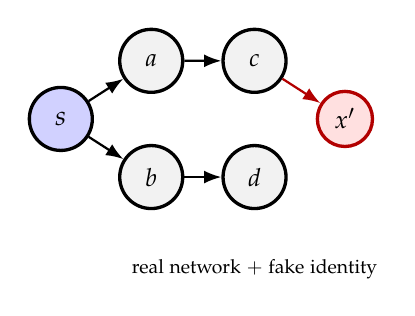
\begin{tikzpicture}[scale=0.82]
  \node[seller] (s) at (0,1.4) {$s$};
  \node[buyer] (a) at (1.4,2.3) {$a$};
  \node[buyer] (b) at (1.4,0.5) {$b$};
  \node[buyer] (c) at (3.0,2.3) {$c$};
  \node[buyer] (d) at (3.0,0.5) {$d$};
  \node[sybil] (x) at (4.4,1.4) {$x'$};
  \draw[arrow] (s)--(a); \draw[arrow] (s)--(b);
  \draw[arrow] (a)--(c); \draw[arrow] (b)--(d);
  \draw[redarrow] (c)--(x);
  \node[below=5mm of d, align=center, font=\scriptsize] {real network $+$ fake identity};
\end{tikzpicture}
\end{column}
\end{columns}
\vspace{1mm}
\greenblock{Main message}{Diffusion mechanisms reward invitation, but the same reward structure can be exploited by fake identities. We propose a restricted, explicit way to lift Sybil robustness to multi-item GIDM.}
\end{frame}

% -----------------------------------------------------------------------------
\begin{frame}{Single-item auction in a social network}
\begin{columns}[T,totalwidth=\textwidth]
\begin{column}{0.48\textwidth}
\centering
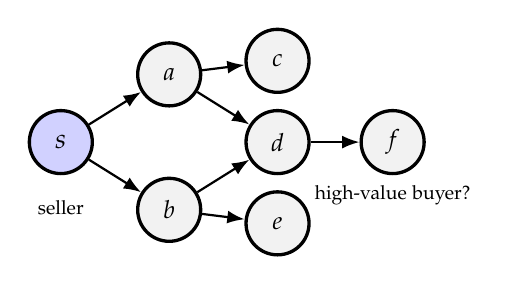
\begin{tikzpicture}[scale=0.86]
  \node[seller] (s) at (0,0) {$s$};
  \node[buyer] (a) at (1.6,1.0) {$a$};
  \node[buyer] (b) at (1.6,-1.0) {$b$};
  \node[buyer] (c) at (3.2,1.2) {$c$};
  \node[buyer] (d) at (3.2,0.0) {$d$};
  \node[buyer] (e) at (3.2,-1.2) {$e$};
  \node[buyer] (f) at (4.9,0.0) {$f$};
  \draw[arrow] (s)--(a); \draw[arrow] (s)--(b);
  \draw[arrow] (a)--(c); \draw[arrow] (a)--(d);
  \draw[arrow] (b)--(d); \draw[arrow] (b)--(e);
  \draw[arrow] (d)--(f);
  \node[below=2mm of s] {\scriptsize seller};
  \node[below=0mm of f] {\scriptsize high-value buyer?};
\end{tikzpicture}
\end{column}
\begin{column}{0.50\textwidth}
\begin{itemize}
    \item Seller knows only her neighbors.
    \item A buyer participates only if auction information reaches her.
    \item Each informed buyer reports
    \[
        a_i=(b_i, r_i'), \qquad r_i'\subseteq r_i.
    \]
    \item Mechanism must incentivize two things:
    \begin{itemize}
        \item truthful valuation report,
        \item forwarding to all neighbors.
    \end{itemize}
\end{itemize}
\question{Problem: why would a buyer invite future competitors?}
\end{column}
\end{columns}
\vspace{-2mm}
{\tiny Baseline model: Li, Hao, Zhao, Zhou, \emph{Mechanism Design in Social Networks}, AAAI 2017.}
\end{frame}

% -----------------------------------------------------------------------------
\begin{frame}{Baseline properties we care about}
\begin{columns}[T,totalwidth=\textwidth]
\begin{column}{0.48\textwidth}
\greenblock{Incentive Compatibility (IC)}{
Truthful bidding and full diffusion is a dominant strategy:
\[
 u_i(v_i,r_i; a_{-i}) \ge u_i(b_i,r_i'; a_{-i}).
\]
}
\greenblock{Individual Rationality (IR)}{
A truthful participant gets non-negative utility.
}
\end{column}
\begin{column}{0.48\textwidth}
\greenblock{Weak Budget Balance / Non-deficit}{
Seller revenue is non-negative:
\[
\sum_i p_i(a) \ge 0.
\]
}
\greenblock{Social welfare}{
For one item, welfare is value of the winner. For $k$ items, sum of values of real winners.
}
\end{column}
\end{columns}
\vspace{3mm}
\begin{center}
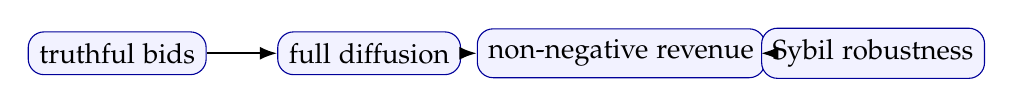
\begin{tikzpicture}
  \node[idea] (ic) at (0,0) {truthful bids};
  \node[idea] (diff) at (3.2,0) {full diffusion};
  \node[idea] (rev) at (6.4,0) {non-negative revenue};
  \node[idea] (rob) at (9.6,0) {Sybil robustness};
  \draw[arrow] (ic)--(diff); \draw[arrow] (diff)--(rev); \draw[arrow] (rev)--(rob);
\end{tikzpicture}
\end{center}
\end{frame}

% -----------------------------------------------------------------------------
\begin{frame}{Two single-item mechanisms: VCG and IDM}
\begin{columns}[T,totalwidth=\textwidth]
\begin{column}{0.49\textwidth}
\begin{block}{Network VCG}
\begin{itemize}
    \item Allocates to highest reachable bidder.
    \item Critical intermediates may receive rewards.
    \item Efficient and IC.
    \item But seller can run a deficit.
\end{itemize}
\end{block}
\end{column}
\begin{column}{0.49\textwidth}
\begin{block}{IDM}
\begin{itemize}
    \item Uses diffusion critical sequence.
    \item Rewards only price-improving diffusion.
    \item IC, IR, non-deficit.
    \item May sacrifice welfare compared with VCG.
\end{itemize}
\end{block}
\end{column}
\end{columns}
\vspace{2mm}
\begin{center}
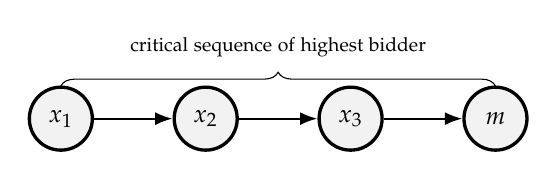
\begin{tikzpicture}[scale=0.92]
  \node[buyer] (x1) at (0,0) {$x_1$};
  \node[buyer] (x2) at (2,0) {$x_2$};
  \node[buyer] (x3) at (4,0) {$x_3$};
  \node[buyer] (m) at (6,0) {$m$};
  \draw[arrow] (x1)--(x2); \draw[arrow] (x2)--(x3); \draw[arrow] (x3)--(m);
  \draw[decorate,decoration={brace,amplitude=5pt},yshift=0.45cm] (0,0)--(6,0) node[midway,yshift=0.5cm] {\scriptsize critical sequence of highest bidder};
\end{tikzpicture}
\end{center}
{\tiny Baseline result: VCG is IC/IR but not weakly budget balanced; IDM is IC/IR and weakly budget balanced.}
\end{frame}

% -----------------------------------------------------------------------------
\begin{frame}{Toy example: VCG can create seller deficit}
\begin{columns}[T,totalwidth=\textwidth]
\begin{column}{0.53\textwidth}
\centering
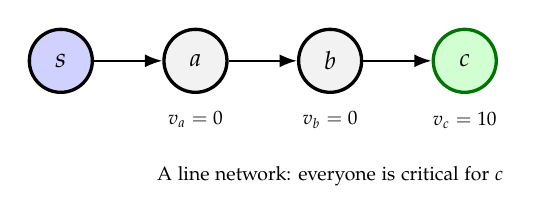
\begin{tikzpicture}[scale=0.95]
  \node[seller] (s) at (0,0) {$s$};
  \tikzbuyer{a}{1.8,0}{$a$}{$v_a=0$}
  \tikzbuyer{b}{3.6,0}{$b$}{$v_b=0$}
  \node[winner] (c) at (5.4,0) {$c$}; \node[below=1mm of c] {\scriptsize $v_c=10$};
  \draw[arrow] (s)--(a); \draw[arrow] (a)--(b); \draw[arrow] (b)--(c);
  \node[below=8mm of b, align=center, font=\scriptsize] {A line network: everyone is critical for $c$};
\end{tikzpicture}
\end{column}
\begin{column}{0.45\textwidth}
\begin{table}
\centering
\small
\begin{tabular}{lcc}
\hline
Mechanism & Winner & Seller revenue \\
\hline
Network VCG & $c$ & $-20$ \\
IDM & $a$ & $0$ \\
\hline
\end{tabular}
\end{table}
\begin{itemize}
    \item In VCG, $c$ pays $0$.
    \item Intermediates $a,b$ each receive reward $10$.
    \item Revenue $=0-10-10=-20$.
    \item IDM avoids deficit by not fully chasing efficiency.
\end{itemize}
\end{column}
\end{columns}
\greenblock{Takeaway}{Diffusion rewards are necessary for reach, but uncontrolled rewards can bankrupt the seller.}
\end{frame}

% -----------------------------------------------------------------------------
\begin{frame}{What remains challenging even after IDM?}
\begin{columns}[T,totalwidth=\textwidth]
\begin{column}{0.48\textwidth}
\begin{block}{Mechanism-design challenges}
\begin{itemize}
    \item Efficiency vs seller revenue
    \item Rewarding intermediates fairly
    \item Extending from one item to many items
    \item Handling strategic graph manipulation
\end{itemize}
\end{block}
\end{column}
\begin{column}{0.48\textwidth}
\begin{alertblock}{New issue: fake identities}
\begin{itemize}
    \item The graph is reported by agents.
    \item A buyer can create fake nodes.
    \item Fake nodes may become ``critical''.
    \item Then diffusion rewards become attack surface.
\end{itemize}
\end{alertblock}
\end{column}
\end{columns}
\vspace{3mm}
\begin{center}
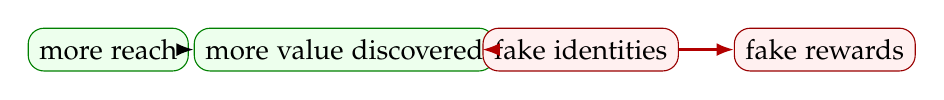
\begin{tikzpicture}
  \node[good] (reach) at (0,0) {more reach};
  \node[good] (value) at (3,0) {more value discovered};
  \node[bad] (fake) at (6,0) {fake identities};
  \node[bad] (reward) at (9.1,0) {fake rewards};
  \draw[arrow] (reach)--(value); \draw[redarrow] (value)--(fake); \draw[redarrow] (fake)--(reward);
\end{tikzpicture}
\end{center}
\end{frame}

% -----------------------------------------------------------------------------
\section{Sybil attacks}

\begin{frame}{What is a Sybil attack?}
\begin{columns}[T,totalwidth=\textwidth]
\begin{column}{0.50\textwidth}
\centering
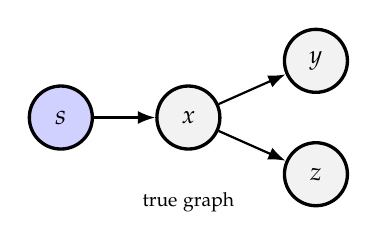
\begin{tikzpicture}[scale=0.9]
  \node[seller] (s) at (0,0) {$s$};
  \node[buyer] (x) at (1.8,0) {$x$};
  \node[buyer] (y) at (3.6,0.8) {$y$};
  \node[buyer] (z) at (3.6,-0.8) {$z$};
  \draw[arrow] (s)--(x); \draw[arrow] (x)--(y); \draw[arrow] (x)--(z);
  \node[below=4mm of x] {\scriptsize true graph};
\end{tikzpicture}
\vspace{3mm}
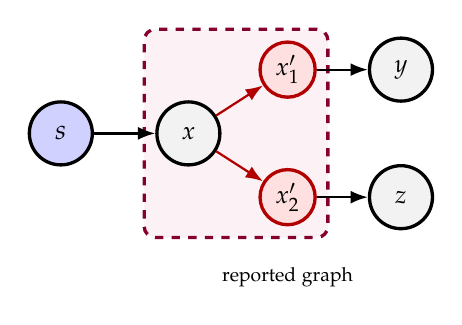
\begin{tikzpicture}[scale=0.9]
  \node[seller] (s) at (0,0) {$s$};
  \node[buyer] (x) at (1.8,0) {$x$};
  \node[sybil] (x1) at (3.2,0.9) {$x_1'$};
  \node[sybil] (x2) at (3.2,-0.9) {$x_2'$};
  \node[buyer] (y) at (4.8,0.9) {$y$};
  \node[buyer] (z) at (4.8,-0.9) {$z$};
  \draw[arrow] (s)--(x); \draw[redarrow] (x)--(x1); \draw[redarrow] (x)--(x2);
  \draw[arrow] (x1)--(y); \draw[arrow] (x2)--(z);
  \begin{scope}[on background layer]
    \node[cluster, fit=(x) (x1) (x2)] {};
  \end{scope}
  \node[below=4mm of x2] {\scriptsize reported graph};
\end{tikzpicture}
\end{column}
\begin{column}{0.48\textwidth}
\begin{itemize}
    \item A real buyer creates fake identities.
    \item Fakes can connect internally or to the creator's neighbors.
    \item No collusion: fakes are controlled by one real buyer.
    \item Goal: increase allocation chance or payment/reward.
\end{itemize}
\greenblock{In diffusion auctions}{Sybil nodes can manipulate the very paths used to define criticality and rewards.}
\end{column}
\end{columns}
{\tiny Sybil model follows Chen, Deng, Wang, Wu, Zhao, \emph{Sybil-Proof Diffusion Auction in Social Networks}, AAMAS 2023.}
\end{frame}

% -----------------------------------------------------------------------------
\begin{frame}{Sybil attack on the toy example: VCG breaks immediately}
\begin{columns}[T,totalwidth=\textwidth]
\begin{column}{0.52\textwidth}
\centering
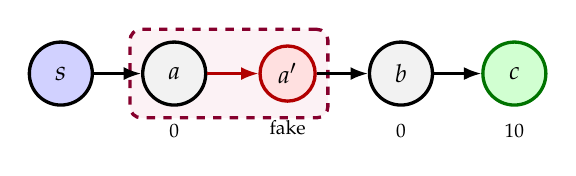
\begin{tikzpicture}[scale=0.9]
  \node[seller] (s) at (0,0) {$s$};
  \node[buyer] (a) at (1.6,0) {$a$};
  \node[sybil] (a1) at (3.2,0) {$a'$};
  \node[buyer] (b) at (4.8,0) {$b$};
  \node[winner] (c) at (6.4,0) {$c$};
  \draw[arrow] (s)--(a); \draw[redarrow] (a)--(a1); \draw[arrow] (a1)--(b); \draw[arrow] (b)--(c);
  \node[below=1mm of a] {\scriptsize $0$};
  \node[below=1mm of a1] {\scriptsize fake};
  \node[below=1mm of b] {\scriptsize $0$};
  \node[below=1mm of c] {\scriptsize $10$};
  \begin{scope}[on background layer]
    \node[cluster, fit=(a) (a1)] {};
  \end{scope}
\end{tikzpicture}
\end{column}
\begin{column}{0.46\textwidth}
\begin{itemize}
    \item Without fake $a'$: $a$ and $b$ are critical for $c$.
    \item With fake $a'$: $a'$ also appears critical.
    \item VCG pays one more diffusion reward.
    \item Since $a$ controls $a'$, her total reward increases.
\end{itemize}
\begin{alertblock}{Failure mode}
VCG rewards graph positions. Fake graph positions create fake rewards.
\end{alertblock}
\end{column}
\end{columns}
\end{frame}

% -----------------------------------------------------------------------------
\begin{frame}{Sybil attack on IDM: changing the critical sequence}
\begin{columns}[T,totalwidth=\textwidth]
\begin{column}{0.55\textwidth}
\centering
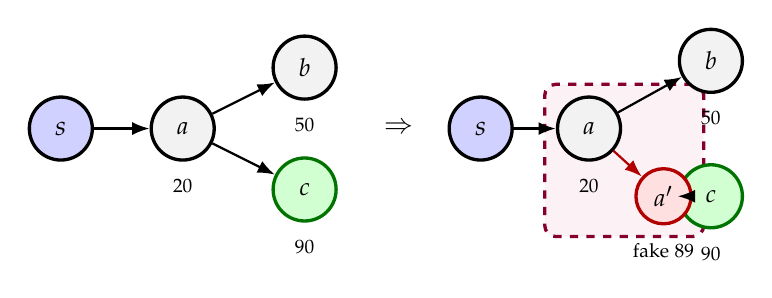
\begin{tikzpicture}[scale=0.86]
  \node[seller] (s) at (0,0) {$s$};
  \node[buyer] (a) at (1.8,0) {$a$};
  \node[buyer] (b) at (3.6,0.9) {$b$};
  \node[winner] (c) at (3.6,-0.9) {$c$};
  \draw[arrow] (s)--(a); \draw[arrow] (a)--(b); \draw[arrow] (a)--(c);
  \node[below=1mm of a] {\scriptsize $20$};
  \node[below=1mm of b] {\scriptsize $50$};
  \node[below=1mm of c] {\scriptsize $90$};
  \node at (5.0,0) {$\Rightarrow$};
  \node[seller] (s2) at (6.2,0) {$s$};
  \node[buyer] (a2) at (7.8,0) {$a$};
  \node[buyer] (b2) at (9.6,1.0) {$b$};
  \node[winner] (c2) at (9.6,-1.0) {$c$};
  \node[sybil] (a1) at (8.9,-1.0) {$a'$};
  \draw[arrow] (s2)--(a2); \draw[arrow] (a2)--(b2); \draw[redarrow] (a2)--(a1); \draw[arrow] (a1)--(c2);
  \node[below=1mm of a2] {\scriptsize $20$};
  \node[below=1mm of b2] {\scriptsize $50$};
  \node[below=1mm of a1] {\scriptsize fake $89$};
  \node[below=1mm of c2] {\scriptsize $90$};
  \begin{scope}[on background layer]
    \node[cluster, fit=(a2) (a1)] {};
  \end{scope}
\end{tikzpicture}
\end{column}
\begin{column}{0.43\textwidth}
\begin{itemize}
    \item IDM uses critical sequence and benchmark bids.
    \item A fake high-bid neighbor can raise the benchmark seen by the winner.
    \item The creator can benefit through changed payments/rewards.
\end{itemize}
\greenblock{Known fact}{Existing diffusion mechanisms such as VCG and IDM are not Sybil-proof.}
\vspace{-1mm}
{\tiny This is the same attack pattern used in the Sybil-proof diffusion auction paper: fake nodes change payments while the real creator controls them.}
\end{column}
\end{columns}
\end{frame}

% -----------------------------------------------------------------------------
\begin{frame}{Definition: Sybil-proofness}
\begin{definition}[Sybil-proofness, informal]
A mechanism is \impterm{Sybil-proof} if a buyer cannot increase her utility by replacing herself with a set of fake identities.
\end{definition}
\vspace{2mm}
\greenblock{Formal shape}{For every real buyer $x$, every profile of others $\theta_{-x}$, and every Sybil attack $\sigma_x$,
\[
    u_x(\text{truthful }x,\theta_{-x})
    \ge
    u_x(\text{identities created by }\sigma_x,\theta_{-x}).
\]
}
\begin{columns}[T,totalwidth=\textwidth]
\begin{column}{0.48\textwidth}
\begin{itemize}
    \item Utility aggregates all identities controlled by $x$.
    \item Fakes may bid and diffuse strategically.
\end{itemize}
\end{column}
\begin{column}{0.48\textwidth}
\begin{itemize}
    \item No collusion between different real buyers.
    \item This is still a strong requirement.
\end{itemize}
\end{column}
\end{columns}
\end{frame}

% -----------------------------------------------------------------------------
\section{Single-item Sybil-proof mechanisms}

\begin{frame}{Can single-item diffusion auctions be made Sybil-proof?}
\begin{columns}[T,totalwidth=\textwidth]
\begin{column}{0.49\textwidth}
\begin{block}{STM: Sybil Tax Mechanism}
\begin{itemize}
    \item Identifies trusted/non-Sybil roots.
    \item Makes suspicious diffusion less profitable.
    \item Strong revenue behavior.
    \item Weaker diffusion incentive to suspicious parts.
\end{itemize}
\end{block}
\end{column}
\begin{column}{0.49\textwidth}
\begin{block}{SCM: Sybil Cluster Mechanism}
\begin{itemize}
    \item Selects/uses a graph structure to limit fake influence.
    \item Credits reachability to selected real agents.
    \item Better diffusion motivation.
    \item Mild welfare/revenue sacrifice.
\end{itemize}
\end{block}
\end{column}
\end{columns}
\vspace{2mm}
\question{Can we transfer this idea to multiple items?}
{\tiny Chen et al. propose STM and SCM for the single-item setting and explicitly leave multi-item Sybil-proof diffusion auctions as an open problem.}
\end{frame}

% -----------------------------------------------------------------------------
\begin{frame}{STM vs SCM: useful intuition for our extension}
\centering
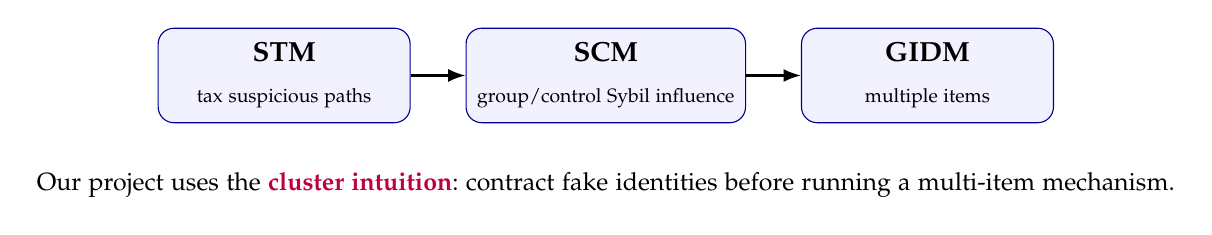
\begin{tikzpicture}[scale=0.95]
  \node[idea, minimum width=3.2cm, minimum height=1.2cm] (stm) at (0,0) {\textbf{STM}\\[1mm]\scriptsize tax suspicious paths};
  \node[idea, minimum width=3.2cm, minimum height=1.2cm] (scm) at (4.3,0) {\textbf{SCM}\\[1mm]\scriptsize group/control Sybil influence};
  \node[idea, minimum width=3.2cm, minimum height=1.2cm] (gidm) at (8.6,0) {\textbf{GIDM}\\[1mm]\scriptsize multiple items};
  \draw[arrow] (stm)--(scm);
  \draw[arrow] (scm)--(gidm);
  \node[below=5mm of scm, align=center, font=\small] {Our project uses the \impterm{cluster intuition}:\ contract fake identities before running a multi-item mechanism.};
\end{tikzpicture}
\vspace{4mm}
\begin{table}
\centering
\small
\begin{tabular}{lccc}
\hline
Mechanism & Single item & Sybil-proof & Multiple items \\
\hline
IDM & yes & no & no \\
STM/SCM & yes & yes & no \\
GIDM & no & no & yes \\
Our SC-GIDM & no & under assumptions & yes \\
\hline
\end{tabular}
\end{table}
\end{frame}

% -----------------------------------------------------------------------------
\section{Moving to multiple items}

\begin{frame}{Multiple homogeneous items: GIDM}
\begin{columns}[T,totalwidth=\textwidth]
\begin{column}{0.52\textwidth}
\centering
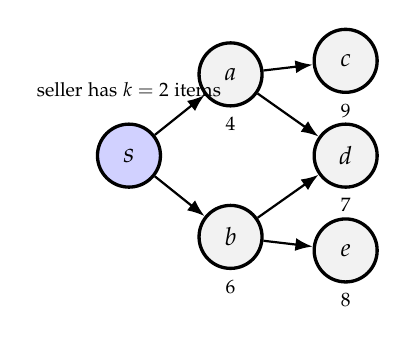
\begin{tikzpicture}[scale=0.86]
  \node[seller] (s) at (0,0) {$s$};
  \node[buyer] (a) at (1.5,1.2) {$a$}; \node[below=0mm of a] {\scriptsize 4};
  \node[buyer] (b) at (1.5,-1.2) {$b$}; \node[below=0mm of b] {\scriptsize 6};
  \node[buyer] (c) at (3.2,1.4) {$c$}; \node[below=0mm of c] {\scriptsize 9};
  \node[buyer] (d) at (3.2,0) {$d$}; \node[below=0mm of d] {\scriptsize 7};
  \node[buyer] (e) at (3.2,-1.4) {$e$}; \node[below=0mm of e] {\scriptsize 8};
  \draw[arrow] (s)--(a); \draw[arrow] (s)--(b);
  \draw[arrow] (a)--(c); \draw[arrow] (a)--(d); \draw[arrow] (b)--(d); \draw[arrow] (b)--(e);
  \node[above=2mm of s] {\scriptsize seller has $k=2$ items};
\end{tikzpicture}
\end{column}
\begin{column}{0.46\textwidth}
\begin{itemize}
    \item GIDM extends IDM to $k$ homogeneous items.
    \item Each buyer needs at most one item.
    \item It uses a winner set and critical diffusion structure.
    \item It preserves IC and IR in the multi-item diffusion model.
    \item Seller revenue is guaranteed better than no advertising baseline.
\end{itemize}
\end{column}
\end{columns}
{\tiny Source: Zhao, Li, Xu, Hao, Jennings, \emph{Selling Multiple Items via Social Networks}, AAMAS 2018.}
\end{frame}

% -----------------------------------------------------------------------------
\begin{frame}{Why ordinary GIDM is not enough under Sybil attacks}
\begin{columns}[T,totalwidth=\textwidth]
\begin{column}{0.56\textwidth}
\centering
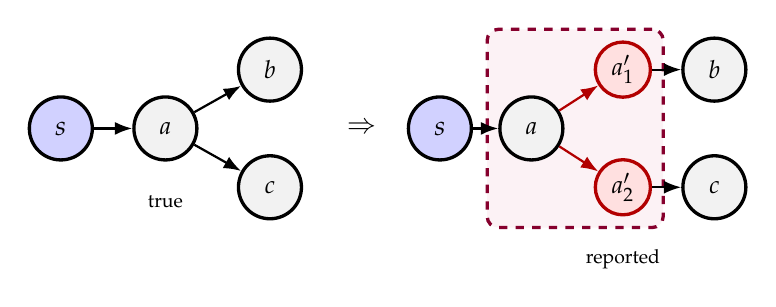
\begin{tikzpicture}[scale=0.83]
  \node[seller] (s) at (0,0) {$s$};
  \node[buyer] (a) at (1.6,0) {$a$};
  \node[buyer] (b) at (3.2,0.9) {$b$};
  \node[buyer] (c) at (3.2,-0.9) {$c$};
  \draw[arrow] (s)--(a); \draw[arrow] (a)--(b); \draw[arrow] (a)--(c);
  \node[below=3mm of a] {\scriptsize true};
  \node at (4.6,0) {$\Rightarrow$};
  \node[seller] (s2) at (5.8,0) {$s$};
  \node[buyer] (a2) at (7.2,0) {$a$};
  \node[sybil] (a1) at (8.6,0.9) {$a_1'$};
  \node[sybil] (a2s) at (8.6,-0.9) {$a_2'$};
  \node[buyer] (b2) at (10.0,0.9) {$b$};
  \node[buyer] (c2) at (10.0,-0.9) {$c$};
  \draw[arrow] (s2)--(a2); \draw[redarrow] (a2)--(a1); \draw[redarrow] (a2)--(a2s);
  \draw[arrow] (a1)--(b2); \draw[arrow] (a2s)--(c2);
  \begin{scope}[on background layer]
    \node[cluster, fit=(a2) (a1) (a2s)] {};
  \end{scope}
  \node[below=3mm of a2s] {\scriptsize reported};
\end{tikzpicture}
\end{column}
\begin{column}{0.42\textwidth}
\begin{itemize}
    \item GIDM treats reported identities as separate buyers.
    \item Fake nodes can alter critical paths.
    \item With $k>1$, fake identities can also affect allocation capacity and price thresholds.
\end{itemize}
\begin{alertblock}{Key observation}
Since $k=1$ is a special case, any multi-item extension that contains IDM-like behavior is not automatically Sybil-proof.
\end{alertblock}
\end{column}
\end{columns}
\end{frame}

% -----------------------------------------------------------------------------
\begin{frame}{Our goal: Sybil robustness for multi-item diffusion}
\begin{center}
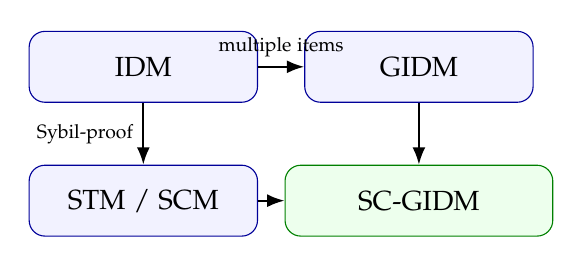
\begin{tikzpicture}[scale=1.0]
  \node[idea, minimum width=2.9cm, minimum height=0.9cm] (single) at (0,0) {IDM};
  \node[idea, minimum width=2.9cm, minimum height=0.9cm] (multi) at (3.5,0) {GIDM};
  \node[idea, minimum width=2.9cm, minimum height=0.9cm] (sp) at (0,-1.7) {STM / SCM};
  \node[good, minimum width=3.4cm, minimum height=0.9cm] (ours) at (3.5,-1.7) {SC-GIDM};
  \draw[arrow] (single)-- node[above, font=\scriptsize] {multiple items} (multi);
  \draw[arrow] (single)-- node[left, font=\scriptsize] {Sybil-proof} (sp);
  \draw[arrow] (multi)--(ours);
  \draw[arrow] (sp)--(ours);
\end{tikzpicture}
\end{center}
\vspace{2mm}
\greenblock{Research question}{Can we combine GIDM with the cluster idea from Sybil-proof single-item auctions to get a meaningful multi-item Sybil-robust mechanism?}
\begin{itemize}
    \item We do \textbf{not} claim to solve arbitrary Sybil detection.
    \item We prove a clean result under certified/non-Sybil roots or perfect clustering.
    \item Then simulations test robustness when clustering is noisy.
\end{itemize}
\end{frame}

% -----------------------------------------------------------------------------
\section{Our mechanism}

\begin{frame}{SC-GIDM: Sybil-Cluster GIDM}
\begin{columns}[T,totalwidth=\textwidth]
\begin{column}{0.52\textwidth}
\centering
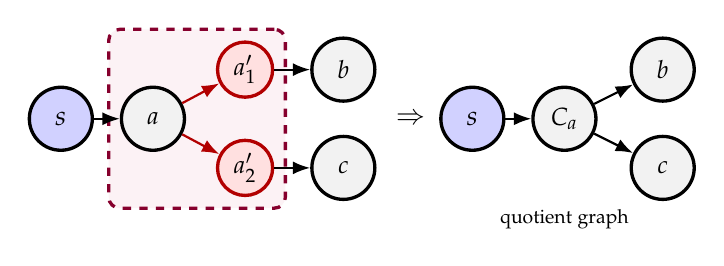
\begin{tikzpicture}[scale=0.78]
  \node[seller] (s) at (0,0) {$s$};
  \node[buyer] (a) at (1.5,0) {$a$};
  \node[sybil] (a1) at (3.0,0.8) {$a_1'$};
  \node[sybil] (a2) at (3.0,-0.8) {$a_2'$};
  \node[buyer] (b) at (4.6,0.8) {$b$};
  \node[buyer] (c) at (4.6,-0.8) {$c$};
  \draw[arrow] (s)--(a); \draw[redarrow] (a)--(a1); \draw[redarrow] (a)--(a2);
  \draw[arrow] (a1)--(b); \draw[arrow] (a2)--(c);
  \begin{scope}[on background layer]
    \node[cluster, fit=(a) (a1) (a2)] (cl) {};
  \end{scope}
  \node at (5.7,0) {$\Rightarrow$};
  \node[seller] (qs) at (6.7,0) {$s$};
  \node[buyer] (qa) at (8.2,0) {$C_a$};
  \node[buyer] (qb) at (9.8,0.8) {$b$};
  \node[buyer] (qc) at (9.8,-0.8) {$c$};
  \draw[arrow] (qs)--(qa); \draw[arrow] (qa)--(qb); \draw[arrow] (qa)--(qc);
  \node[below=6mm of qa, align=center, font=\scriptsize] {quotient graph};
\end{tikzpicture}
\end{column}
\begin{column}{0.46\textwidth}
\begin{enumerate}
    \item Partition identities into clusters.
    \item Contract each cluster into one super-node.
    \item Cluster bid: $B_C=\max_{x\in C} b_x$.
    \item Cluster demand: at most one item.
    \item Run GIDM on the quotient graph.
\end{enumerate}
\end{column}
\end{columns}
\greenblock{Intuition}{Fake identities can exist inside a cluster, but they cannot create extra capacity or extra diffusion positions after contraction.}
\end{frame}

% -----------------------------------------------------------------------------
\begin{frame}{Assumptions: what exactly are we proving?}
\begin{columns}[T,totalwidth=\textwidth]
\begin{column}{0.49\textwidth}
\begin{block}{Auction side}
\begin{itemize}
    \item $k$ homogeneous items.
    \item Single-unit demand.
    \item Quasi-linear utilities.
    \item No collusion between real buyers.
\end{itemize}
\end{block}
\end{column}
\begin{column}{0.49\textwidth}
\begin{block}{Sybil side}
\begin{itemize}
    \item Fake identities are controlled by one buyer.
    \item Fakes have no incoming edges except through creator/fakes.
    \item Perfect cluster oracle for theorem.
    \item Noisy clusters only in simulations.
\end{itemize}
\end{block}
\end{column}
\end{columns}
\vspace{2mm}
\begin{alertblock}{Important honesty point}
We are not solving the general Sybil detection problem. We are proving that \emph{if} a trusted-root / cluster layer is available, then GIDM can be lifted safely in a restricted multi-item model.
\end{alertblock}
\end{frame}

% -----------------------------------------------------------------------------
\begin{frame}{Main theorem package}
\begin{theorem}[Reduction]
Under perfect clustering, SC-GIDM on the reported graph is outcome-equivalent to GIDM on the true real-agent graph.
\end{theorem}
\vspace{-1mm}
\begin{proof}[Proof idea]
All identities of a real buyer contract into one cluster. Internal fake paths vanish. No fake can create a new real incoming edge. Hence the quotient graph has the same real reachability structure.
\end{proof}
\vspace{1mm}
\greenblock{Consequences}{
\begin{itemize}
    \item IR and IC transfer from GIDM on the quotient graph.
    \item Non-deficit / seller-revenue guarantees transfer from GIDM.
    \item Sybil-proofness follows because fake identities do not change the quotient instance.
\end{itemize}
}
\end{frame}

% -----------------------------------------------------------------------------
\begin{frame}{Why this blocks the earlier attack}
\begin{columns}[T,totalwidth=\textwidth]
\begin{column}{0.54\textwidth}
\centering
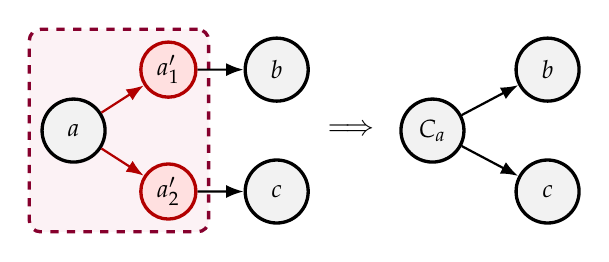
\begin{tikzpicture}[scale=0.86]
  \node[buyer] (a) at (0,0) {$a$};
  \node[sybil] (a1) at (1.4,0.9) {$a_1'$};
  \node[sybil] (a2) at (1.4,-0.9) {$a_2'$};
  \node[buyer] (b) at (3.0,0.9) {$b$};
  \node[buyer] (c) at (3.0,-0.9) {$c$};
  \draw[redarrow] (a)--(a1); \draw[redarrow] (a)--(a2); \draw[arrow] (a1)--(b); \draw[arrow] (a2)--(c);
  \begin{scope}[on background layer]
    \node[cluster, fit=(a) (a1) (a2)] {};
  \end{scope}
  \node at (4.1,0) {$\Longrightarrow$};
  \node[buyer] (ca) at (5.3,0) {$C_a$};
  \node[buyer] (bb) at (7.0,0.9) {$b$};
  \node[buyer] (cc) at (7.0,-0.9) {$c$};
  \draw[arrow] (ca)--(bb); \draw[arrow] (ca)--(cc);
\end{tikzpicture}
\end{column}
\begin{column}{0.44\textwidth}
\begin{itemize}
    \item Multiple fake bids become one effective cluster bid.
    \item Multiple fake positions become one graph position.
    \item Cluster receives at most one item.
    \item Internal fake diffusion earns no separate reward.
\end{itemize}
\greenblock{Therefore}{The attack has no additional strategic degree of freedom beyond the real buyer's cluster-level report.}
\end{column}
\end{columns}
\end{frame}

% -----------------------------------------------------------------------------
\section{Experiments and discussion}

\begin{frame}{Simulation plan: what we compare}
\begin{columns}[T,totalwidth=\textwidth]
\begin{column}{0.48\textwidth}
\begin{block}{Mechanisms}
\begin{itemize}
    \item Local $k$-Vickrey: no diffusion.
    \item GIDM: no Sybil defense.
    \item GIDM under Sybil attacks.
    \item SC-GIDM: cluster then run GIDM.
    \item Oracle GIDM on true graph.
\end{itemize}
\end{block}
\end{column}
\begin{column}{0.48\textwidth}
\begin{block}{Networks and attacks}
\begin{itemize}
    \item Path, tree, Erd\H{o}s--R\'enyi, scale-free graphs.
    \item Sybil chain attack.
    \item Sybil star attack.
    \item Fake high-bid threshold attack.
    \item Noisy clustering: false negatives and false positives.
\end{itemize}
\end{block}
\end{column}
\end{columns}
\vspace{2mm}
\greenblock{Main experimental question}{How much welfare/revenue do we sacrifice to reduce attacker gain and fake allocation leakage?}
\end{frame}

% -----------------------------------------------------------------------------
\begin{frame}{Metrics: what counts as ``better''?}
\begin{columns}[T,totalwidth=\textwidth]
\begin{column}{0.50\textwidth}
\begin{itemize}
    \item \impterm{Seller revenue}: $\sum_i p_i$.
    \item \impterm{Real welfare}: value from real winners only.
    \item \impterm{Attacker gain}: utility after attack minus truthful utility.
    \item \impterm{Fake allocation leakage}: fraction of items assigned to fake identities.
\end{itemize}
\end{column}
\begin{column}{0.48\textwidth}
\centering
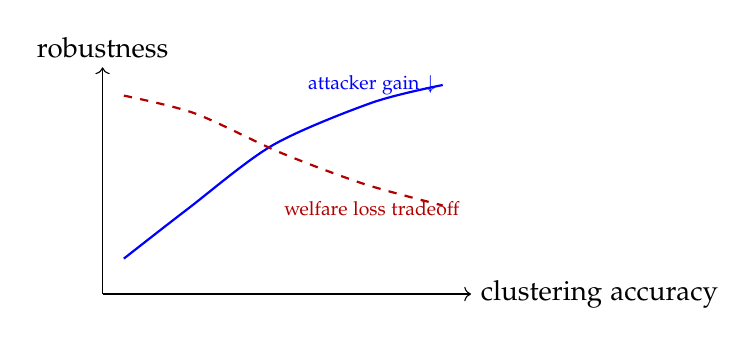
\begin{tikzpicture}[scale=0.9]
  \draw[->] (0,0)--(5.2,0) node[right] {clustering accuracy};
  \draw[->] (0,0)--(0,3.2) node[above] {robustness};
  \draw[thick, blue] plot[smooth] coordinates {(0.3,0.5) (1.2,1.2) (2.4,2.1) (3.8,2.7) (4.8,2.95)};
  \draw[thick, red!70!black, dashed] plot[smooth] coordinates {(0.3,2.8) (1.3,2.55) (2.5,2.0) (3.7,1.55) (4.8,1.25)};
  \node[blue, font=\scriptsize] at (3.8,2.95) {attacker gain $\downarrow$};
  \node[red!70!black, font=\scriptsize] at (3.8,1.2) {welfare loss tradeoff};
\end{tikzpicture}
\vspace{1mm}
{\scriptsize Qualitative tradeoff plot, not a claimed result.}
\end{column}
\end{columns}
\end{frame}

% -----------------------------------------------------------------------------
\begin{frame}{What we expect to learn}
\begin{itemize}
    \item In the no-attack setting, GIDM should usually be better than local sale because diffusion reaches more buyers.
    \item Under Sybil attacks, ordinary GIDM can be manipulated because it runs on reported identities.
    \item SC-GIDM should reduce attacker gain under good clustering.
    \item False negatives hurt robustness; false positives hurt welfare.
    \item Dense graphs may lose less welfare because there are alternate diffusion paths.
\end{itemize}
\vspace{2mm}
\begin{center}
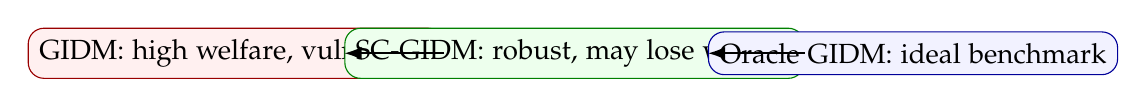
\begin{tikzpicture}
  \node[bad] (gidm) at (0,0) {GIDM: high welfare, vulnerable};
  \node[good] (sc) at (4.3,0) {SC-GIDM: robust, may lose welfare};
  \node[idea] (oracle) at (8.6,0) {Oracle GIDM: ideal benchmark};
  \draw[arrow] (gidm)--(sc); \draw[arrow] (sc)--(oracle);
\end{tikzpicture}
\end{center}
\end{frame}

% -----------------------------------------------------------------------------
\begin{frame}{Limitations and future directions}
\begin{columns}[T,totalwidth=\textwidth]
\begin{column}{0.48\textwidth}
\begin{alertblock}{Limitations}
\begin{itemize}
    \item Perfect clustering is strong.
    \item No collusion between real buyers.
    \item Homogeneous items only.
    \item Single-unit demand only.
    \item Not optimal among all SP mechanisms.
\end{itemize}
\end{alertblock}
\end{column}
\begin{column}{0.48\textwidth}
\begin{block}{Next steps}
\begin{itemize}
    \item Better noisy-cluster guarantees.
    \item Heterogeneous items.
    \item Multi-unit demand.
    \item Fair reward sharing inside clusters.
    \item Compare with STM-like taxes for $k$ items.
\end{itemize}
\end{block}
\end{column}
\end{columns}
\vspace{2mm}
\greenblock{Research-style framing}{We solve a restricted version cleanly, show why the unrestricted version is hard, and evaluate the robustness--welfare tradeoff experimentally.}
\end{frame}

% -----------------------------------------------------------------------------
\begin{frame}{Final takeaway}
\begin{center}
\Large
\textbf{Diffusion auctions need graph incentives.}\\[2mm]
\textbf{Graph incentives create Sybil attack surfaces.}\\[2mm]
\textbf{Cluster reduction is a natural bridge to multi-item Sybil robustness.}
\end{center}
\vspace{5mm}
\begin{columns}[T,totalwidth=\textwidth]
\begin{column}{0.32\textwidth}
\greenblock{Baseline}{IDM/GIDM give diffusion incentives and revenue guarantees.}
\end{column}
\begin{column}{0.32\textwidth}
\greenblock{Issue}{Reported identities can manipulate critical paths and rewards.}
\end{column}
\begin{column}{0.32\textwidth}
\greenblock{Our extension}{Contract Sybil clusters, then run GIDM on the quotient graph.}
\end{column}
\end{columns}
\vspace{4mm}
\begin{center}
\large Thank you. Questions?
\end{center}
\end{frame}

% -----------------------------------------------------------------------------
\begin{frame}{References}
\small
\begin{itemize}
    \item Bin Li, Dong Hao, Dengji Zhao, Tao Zhou. \emph{Mechanism Design in Social Networks}. AAAI 2017.
    \item Dengji Zhao, Bin Li, Junping Xu, Dong Hao, Nicholas R. Jennings. \emph{Selling Multiple Items via Social Networks}. AAMAS 2018.
    \item Hongyin Chen, Xiaotie Deng, Ying Wang, Yue Wu, Dengji Zhao. \emph{Sybil-Proof Diffusion Auction in Social Networks}. AAMAS 2023.
\end{itemize}
\vspace{2mm}
\greenblock{How to read our claims}{All theorem-level claims are for homogeneous items, single-unit demand, no collusion, and perfect Sybil clustering. Simulations explore what happens when the clustering assumption is relaxed.}
\end{frame}

\backmatter

\end{document}
